\section{Fehlerradius}\label{anhang:fehler}
Der maximal zulässige Fehlerradius $\beta$ wird als Winkel zwischen der optimalen sowie der fehlerhaften Bahn
der Kugel definiert, welche eingenommen wird, wenn der Mittelpunkt falsch erkannt oder umgerechnet wurde.
Weiterhin kann in Abbildung \ref{fig:fehlerwinkel} erkannt werden, dass dieser Winkel maximal wird,
wenn der falsch erkannte Mittelpunkt $M'$ orthogonal zur optimalen Bahn liegt,
welche wiederum über den Zielpunkt $T$ und den wirklichen Kugelmittelpunkt $M$ gegeben ist.

\begin{figure}[h!]
    \begin{center}
        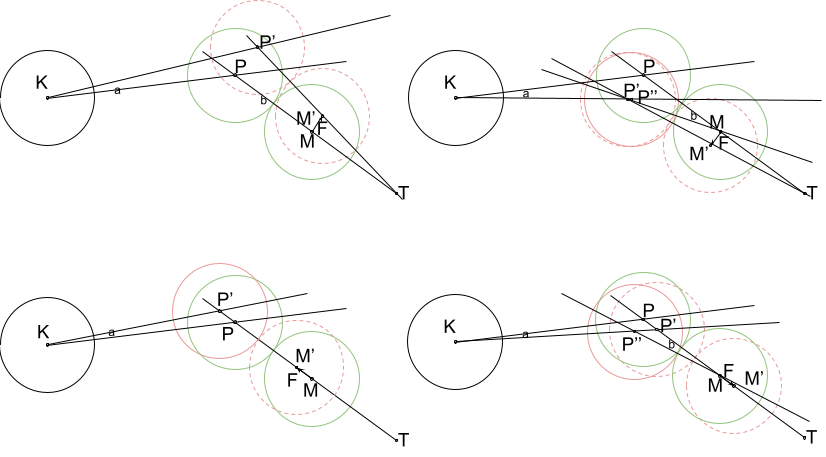
\includegraphics[width=0.7\linewidth]{../common/07_appendix/resources/02_fehlerwinkel.png}
    \end{center}
    \caption{Fehlerwinkel}
    \label{fig:fehlerwinkel}
\end{figure}

Wichtig zu beachten ist auch, dass wenn der Winkel $\beta = 0$ ist, dies nicht bedeutet,
dass kein Fehler aufgetreten ist. In dem Fall wird die Kugel entweder nicht getroffen (Fehler) oder sie wird korrekt
getroffen (kein Fehler).

Sei $M$ die Position des Zielballs, $M'$ die falsch erkannte Position des Zielballs, $\vec{F}$ der Fehlervektor zwischen $M$ und $M'$,
$K$ die Startposition des Spielballs, $P$ die Zielposition des Spielballs, $T$ die Zielposition des Zielballs
und $R$ der Radius einer Kugel, dann gilt:

\begin{align}
    T(T_x, T_y), K(K_x, K_y), M(M_x, M_y), M'(M_x', M_y')\\
    \vec{MK} = K - M\\
    \hat{MK} = \frac{\vec{MK}}{\norm{\vec{MK}}}\\
    P = M + 2 \cdot R \cdot \hat{MK}\\
    M' = M + \vec{F}\\
    \vec{TM'} = M' - T\\
    \hat{TM'} = \frac{\vec{TM'}}{\norm{\vec{TM'}}}\\
    P' = M' + 2 \cdot R \cdot \hat{TM'}\\
\end{align}

Aus Abbildung \ref{fig:fehlerwinkel_vereinfachung} ist ersichtlich, dass der Punkt $P''$ auf der Linie $KP'$ und auf dem
Kreis um den Mittelpunkt $M$ mit dem Radius $2R$ liegt. Daher kann dieser bestimmt werden, indem ein Linie-Kreis-Schnittpunkt
bestimmt wird.

Sei der Kreis $S$ in Normalenform mit dem Kreismittelpunkt $C$, Radius $R$
und die Linie $L$ in Parameterform mit Punkt $P$ und Richtungsvektor $V$ gegeben, dann gilt:

\begin{align}
    S: \norm{X - C}^2 = R^2\\
    L: D = P + t \cdot V\\
    \norm{V} = 1
\end{align}

Nach Einfügen der Liniengleichung in die Kreisgleichung folgt:

\begin{align}
    \norm{P + t \cdot V - C}^2 = R^2\\
    \norm{t \cdot V + P - C}^2 = R^2\\
    \norm{t \cdot V + (P - C)}^2 = R^2\\
    (t \cdot V + (P - C)) \cdot (t \cdot V + (P - C)) = R^2\\
    (t \cdot V) \cdot (t \cdot V + (P - C)) + (P - C) \cdot (t \cdot V + (P - C)) = R^2\\
    (t \cdot V) \cdot (t \cdot V) + (t \cdot V) \cdot (P - C) + (P - C) \cdot (t \cdot V) + (P - C) \cdot (P - C) = R^2\\
    (t^2 \cdot V^2) + 2t \cdot (V \cdot (P - C)) + (P - C)^2 = R^2\\
    (t^2 \cdot V^2) + 2t \cdot (V \cdot (P - C)) + (P - C)^2 - R^2 = 0\\
\end{align}

Es resultiert eine Quadratische Formel, welche nach $t$ gelöst werden muss.
Dazu kann die Mitternachtsformel verwendet werden \cite{wiki.mitternachtsformel:1}.

\begin{align}
    a = V^2 = 1\\
    b = 2 \cdot (V \cdot (P - C))\\
    c = (P - C)^2 - R^2\\
\end{align}

Die Diskriminante der Mitternachtsformel muss beachtet werden, da diese die drei möglichen Ereignisse beschreibt.
Wenn die Diskrimante kleiner als 0 ist, dann ist der Fehler so gross, dass der Zielball nicht mehr getroffen wird.
Ist die Diskriminante gleich 0, so gibt es einen möglichen Schnittpunkt.
Sofern die Diskriminante grösser 0 ist, gibt es zwei Schnittpunke, wovon derjenige mit dem kleineren $t$ gewählt wird.

\begin{align}
t_1 = \frac{-b + \sqrt{b^2 - 4ac}}{2a}\\
t_2 = \frac{-b - \sqrt{b^2 - 4ac}}{2a}\\
t = \min{t_1, t_2}
\end{align}

Nun kann der Punkt $P''$ bestimmt und der Winkel $\beta$ berechnet werden.

\begin{align}
    \vec{KP'} = P' - K\\
    \hat{KP'} = \frac{\vec{KP'}}{\norm{\vec{KP'}}}\\
    P'' = K + t \cdot \hat{KP'}\\
    \vec{MP''} = P'' - M\\
    \hat{MP''} = \frac{\vec{MP''}}{\norm{\vec{MP''}}}\\
    \vec{MP} = P'' - M\\
    \hat{MP} = \frac{\vec{MP}}{\norm{\vec{MP}}}\\
    \beta = \arccos(\hat{MP''} \cdot \hat{MP})
\end{align}

Um die maximale Fehlerdistanz zu bestimmen, wird angenommen, dass eine orthogonale Verschiebung des Kugelmittelpunkts
das Worst-Case-Szenario bildet. Dies wird in Abbildung \ref{fig:fehlerwinkel_vereinfachung} verdeutlicht.

\begin{figure}[h!]
    \begin{center}
        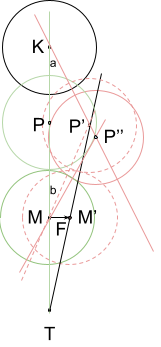
\includegraphics[width=0.2\linewidth]{../common/07_appendix/resources/03_fehlerwinkel_vereinfacht.png}
    \end{center}
    \caption{Fehlerwinkel vereinfacht}
    \label{fig:fehlerwinkel_vereinfachung}
\end{figure}

Es soll nun die Auswirkungen des Fehlervektors $\vec{F}$ des Zielball auf dessen Zielposition $T$ bestimmt werden.
Durch den Fehlervektor entsteht eine inkorrekte Zielposition $T'$. Diese kann über den Winkel $\beta$ wie auch die Distanz $D$ zur
Zielposition $T$ bestimmt werden, siehe Abbildung \ref{fig:abweichung_ueber_distanz}.

\begin{figure}[h!]
    \begin{center}
        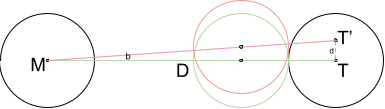
\includegraphics[width=0.4\linewidth]{../common/07_appendix/resources/04_abweichung.png}
    \end{center}
    \caption{Abweichung über Distanz}
    \label{fig:abweichung_ueber_distanz}
\end{figure}

Bei $d$ handelt es sich um die Gegenkathete, bei $D$ um die Ankathete, daher folgt:
\begin{align}
    \tan(\beta) = \frac{d}{D}\\
    d = \tan(\beta) \cdot D
\end{align}

Um die Auswirkung eines Fehlervektors der Länge $2.15mm$ darzustellen, wird die vereinfachte Situation aus Abbildung
\ref{fig:fehlerwinkel_vereinfachung} vorausgesetzt.

Für eine Abweichung um $\vec{F} = \begin{pmatrix}0\\2.15\end{pmatrix}$ auf ein Ziel $T$ der
Entfernung $T = \begin{pmatrix}1800\\0\end{pmatrix}$ mit gegebener Position des Zielballs $M = \begin{pmatrix}100\\0\end{pmatrix}$,
sowie Startposition des Spielballs $K = \begin{pmatrix}0\\0\end{pmatrix}$
ergibt sich ein Winkel $\beta$ von $2.431\deg$. Dies ergibt eine Gesamtabweichung von $d = 72.17mm$.
Es wird davon ausgegangen, dass die Distanzen, welche eine
Kugel zurücklegen, tendenziell kleiner sein werden, da Stösse über grössere Distanzen schwieriger sind.
Daher handelt es sich hierbei um einen Worst-Case.
Angenommen die Distanz $D$ wird halbiert, dann sinkt die Abweichung auf $37.16mm$.

\section{Fehler - Grundwahrheit}\label{anhang:fehler:grundwahrheit}
Als Grundwahrheit zur Bestimmung der Gesamtabweichung in [mm] dient ein manuell annotiertes Testbild.
Auf diesem wird also von einer Person der Kugelmittelpunkt in ganzen Pixeln eruiert. Die Grundwahrheit
ist gegeben durch \ref{eq:8}.
\begin{align}
    G = (G_x, G_y)\label{eq:8}
\end{align}
Weiterhin ist bekannt, wie vielen Millimetern ein Pixel entspricht. Diese Information ist einerseits über die Masse des
Tisches $T$ wie auch über die Auflösung des Bildes $B$ gegeben.
\begin{align}
    T = (T_x, T_y) [mm]\\
    B = (B_x, B_y) [pixel]\\
    TB = (T_x/B_x, T_y/B_y)
\end{align}
Unter der Annahme, dass bei einem Pixel das Zentrum angegeben wird, kann die Abweichung der Detektion $D$ wie in \ref{eq:9}
dargestellt werden.
\begin{align}
    D = (D_x, D_y) [subpixel]\\
    \Delta = TB - D\label{eq:9}
\end{align}
Die Informationen $T$ wie auch $B$ sind gegeben.
$B$ ist die Breite und Höhe des Spielbereichs in Pixel und wurde anhand eines Bildes festgestellt.
\begin{align}
    T = (1881, 943) [mm]\\
    B = (1118.72, 565.284) [pixel]\\
    TB = (1.681, 1.668) [\frac{mm}{pixel}]
\end{align}
Unter der Annhame, dass eine Pixelkoordinate dem Zentrum des Pixels entspricht, der Kugelmittelpunkt
subpixelgenau erkannt wird und als Grundwahrheit das korrekte Pixel angegeben wurde, kann die
maximale Abweichung $\Delta_{\max}$ wie in \ref{eq:10} angegeben werden.
\begin{align}
    \Delta_{\max} = \frac{1 [pixel]}{2} \cdot TB\label{eq:10}\\
    \Delta_{\max} = (0.8405, 0.834) [mm]\\
    \norm{\Delta_{\max}} = \sqrt{0.8405^2 +  0.834^2} = 1.18406 mm
\end{align}
